
\subsection{Martingale Digression}

For a moment we will be formal. Let $(\Omega, \mathcal{A}, \mathbb{P})$ be a measure space. That is $\Omega$ is a fixed set, and $\mathcal{A}$ forms a $\sigma$-algebra of subsets of $\Omega$.

\footnote{Recall that a $\sigma$-algebra if \begin{itemize}\item $\Omega, \emptseyt\in \mathcal{A}$ \item $A\in \mathcal{A} \rightarrow A^c\in \mathcal{A}$ \item For any countable sequence of sets $\{F_i\}_{i=1}^n\subset 2^{\Omega}$, $\cup_{i=1}^n F_i\in \mathcal{A}$. \end{itemize}}

\begin{definition}
We say that $\mathcal{H} = \{\mathcal{H}_i\}_{i=0}^n$ is a filtration if 
\begin{itemize}
    \item $\mathcal{H}_0 = \emptyset $
    \item Each $\mathcal{H}_t\subset \mathcal{A}$
    \item $\mathcal{H}_t\subset \mathcal{H}_{t+1}$
\end{itemize}

A sequence of random variables $\{X_t\}_{t=1}^{\infty}$ is adapted to to $\mathcal{H}$ if $X_t$ is $\mathcal{H}_t$ measurable. 
\end{definition}
Intuitively, the filtration captures all information available to us at each time $t$. Given a collection of random variables $X_1, \dots, X_t, \cdots$, i.e. measurable with respect to $\mathcal{A}$. The most interesting filtrations that we will consider in this class are $\mathcal{H}_t = \sigma\{X_{s}\}_{s=1}^t$ - that is the filtration determined by the random variables. Intuitively, the decisions we make at time $t$ will be dependent on what information we have up to that time. 

\begin{definition}
    Fix some probability space $(\Omega, \mc{A}, \P)$ and a filtration $\mathcal{H} = \{\mathcal{H}_t\}_{t=1}^{\infty}$. We say that an adapted sequence of random variables $\{X_t\}_{t=1}^{\infty}$ is 
    \begin{itemize}
        \item A martingale of $\E[X_{t}|\mb{H}_{t-1}] = X_{t-1}$
        \item A super-martingale of $\E[X_{t}|\mb{H}_{t-1}] \leq X_{t-1}$
        \item A sub-martingale of $\E[X_{t}|\mb{H}_{t-1}] \geq X_{t-1}$
    \end{itemize}    
\end{definition}


\noindent\textbf{Example 1.} Again consider a sequence of random variables $\{X_t\}_{t\geq 1}$ where each $\E[X_{t+1}|X_t] = 0$ (eg iid mean zero random variables). Then define $S_t = X_1+\cdots + X_t$.
\begin{align*}
    \E[S_{t+1}|\{X_t\}_{t=1}^n] = \E[S_{t} + X_{t+1}|X_t] = S_t 
\end{align*}
so $\{S_t\}_{t\geq 1}$ forms a martingal sequence.

\noindent\textbf{Example 2.} Assume that $X_1, \cdots, X_t\sim p_0(X)$ and let $p_1$ be a different distribution. Then $\Lambda_t$ forms a martingale sequence under $p_0$.


\begin{definition}
    We say that a random variable $\tau\in \mathbb{N}\cup \{\infty\}$ is a stopping time with respect to $\mathcal{H} = \{\mathcal{H}_t\}_{t=1}^{\infty}$ if $\{\tau = t\}\in \mathcal{H}_t$.
\end{definition}
Intuitively, a stopping time is a decision on whether to stop or proceed dependent on all the information up to and including time $t$.

INCLUDE INTUITION ON STOPPING TIME BASED ON RANDOM WALK.

\begin{theorem}[Optional Stopping]
If 
\begin{itemize}
\item $\P(\tau < c) = 1$ for some $c$
\item There exists a constant $c$ so that $\E[|X_{t+1} - X_t||\mathcal{F}_t] \leq c$ and $\E[\tau] \leq \infty$.
\end{itemize}
\begin{itemize}
    \item If $X_t$ forms a martingale, $\E[X_t] = \E[X_0]$
    \item If $X_t$ forms a super - martingale, $\E[X_t] \leq \E[X_0]$
    \item If $X_t$ forms a sub - martingale, $\E[X_t] \geq \E[X_0]$
\end{itemize}
\end{theorem}

We will use Doob's optimal stopping several times. However, our first application is an important result in it's own right that we will need for the SPRT, Wald's theorem.

\begin{theorem}[Wald's Theorem]
    Let $\{X_t\}_{t=1}^{\infty}$ be i.i.d. random variables with $\E[X_t] = \mu$. Assume that $\tau$ with $\E[\tau]\leq \infty$ is a stopping time wrt the filtration $\mathcal{F}_{t} = \{X_s\}_{s=1}^t$. Then $\E[\sum_{s=1}^{\tau} X_s] = \mu\E[\tau]$
\end{theorem}
\begin{proof}
    Define the martingale $M_n = \sum_{i=1}^n X_i - \E[X_i]$. By the optional stopping theorem
    \begin{align*}
        \E[M_{\tau}] = \E[S_{\tau} - T_{\tau}] = \E[M_0] = 0
    \end{align*}
    \textit{Exercise.} Show that it is valid to apply the second condition of the optional stopping theorem. 
    
    Subtracting $\E[T_{\tau}] = \mu\E[\tau]$ now gives the result. 
\end{proof}


\begin{theorem}[Ville's Inequality]
    Let $\{X_t\}_{t=1}^{\infty}$ be a family of random variables adapted to the filtration $\mc{F}_t$ with $X_t\geq 0$ almost surely.  If $X_t$ forms a super-martingale, $\P(\max_{t\geq 1} X_t \geq \epsilon) \leq \frac{\E[X_0]}{\epsilon}$
    % \begin{itemize}
    %     \item (Ville's Inequality) If $X_t$ forms a super-martingale, $\P(\max_{t} X_t \geq \epsilon) \leq \frac{\E[X_0]}{\epsilon}$
    %     \item (Maximal Inequality) If $X_t$ forms a sub-martingale, $\P(\max_{t=1,\cdots, N} X_t \geq \epsilon) \leq \frac{\E[X_N]}{\epsilon}$
    % \end{itemize}
\end{theorem}
\begin{proof}
    Define the stopping time $\tau(t) = \min\{t+1,\min\{s\leq t: X_t\geq \epsilon\}\}$ and the event $A_t = \{\sup_{s\leq t} X_t \geq \epsilon\}$. Clearly $\tau(t)$ is a bounded stopping time. Then by Doob's optimal stopping
    \begin{align*}
        \E[X_0] 
        &\geq \E[X_{\tau(t)}] \\
        &\geq \E[X_{\tau(t)} \1\{\tau \leq t\}] \\
        &\geq \epsilon \P(\tau \leq t).
        
    \end{align*}
    Rearranging shows that $\P(\sup_{s\leq t} X_t \geq \epsilon) \leq \frac{\E[X_0]}{\epsilon}$ for all $t\geq 1$. However note that $A_1\subset A_2\subset A_3\subset \cdots$ so $\P(\sup_{t\geq 1} X_{t} > \epsilon) \leq \frac{\E[X_0]}{\epsilon}$.
\end{proof}


\subsection{Always-Valid Confidence Intervals}

Given a sequence of mean-zero independent random variables $X_1, X_2, \cdots$, an $\alpha$-\textit{always-valid} confidence interval is a sequence of bounds $c(t, \alpha)$ such that 
\[\P\left(\left|\frac{1}{t}\sum_{s=1}^t X_i\right| > c(t, \alpha)\right) < \delta.\]

As we saw above, for $1$-subGaussian random variables, $c(t,\alpha) = \sqrt{2\log(2t^2/\delta)/t}$ forms an anytime-confidence bound. The key to developing anytime confidence intervals is given by the following maximal inequailities for martingales.

\noindent\textbf{Line-Cross Inequalities.} Assume that $X_1, X_2, \cdots, $ is a sequence of i.i.d. centered $1$-subGaussian random variables. Define $S_t = \sum_{s=1}^t X_s$ and $M_t = \exp\left(\lambda S_t - \frac{t\lambda^2}{2}\right), t\geq 1, M_0 =1$ Then,
\begin{align*}
    \E[M_t|M_{t-1}] = M_{t-1}\E\left[\exp\left(\lambda X_t - \frac{\lambda^2 t}{2}\right)|M_{t-1}\right] \leq M_{t-1}.
\end{align*}

Then by Ville's inequality,
\begin{align*}
    \P(\max_{t\in \mathbb{N}} M_t \geq \delta) \leq 1/\delta \\
    \iff \P\left(\max_{t\in \mathbb{N}} S_t \geq \frac{\lambda t}{2} +  \frac{\log{1/\delta}}{\lambda}\right) \leq \delta.
\end{align*}



\noindent\textbf{Mixture Sequential Probability Ratio Test}

Let's connect this back to the SPRT. The (one-sided) SPRT (at least in the case of a mean-0 Gaussian) of $H_0:\mu = 0$ vs $H_1:\mu = \Delta$, guaranteed that with probability greater than $1-\delta$, if there exists a time $t$ such that
\[S_t \geq \frac{\lambda \Delta}{2} +  \frac{\log{1/\delta}}{\Delta}\]
we should return $H_1$. We also saw this test was optimal in the sense that if $H_1$ is true the expected hitting time of this boundary is minimized. 

There is a nice geometric connection between the family of linear-crossing boundaries given above and the fixed-time Chernoff bound $\sqrt{2\log(1/\delta)/t}$. Namely, the line $\Delta t/2+ \log(1/\delta)/t$ is tangent to the Chernoff at precisely the expected stopping time $t = 2\log(1/\delta)/\Delta^2$!

\begin{figure}
    \centering
    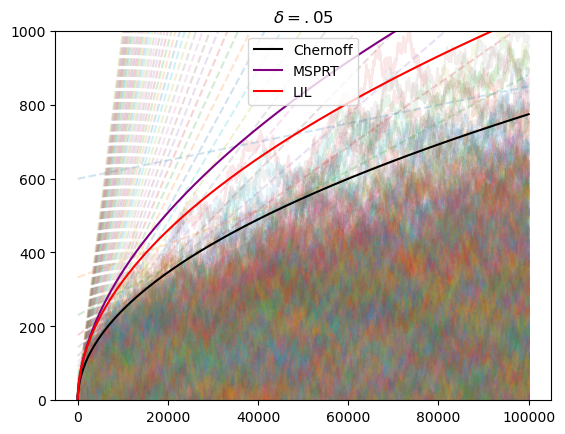
\includegraphics{boundaries.png}
    \caption{Chernoff, MSPRT, and LIL boundaries. Note that the Chernoff boundary is the pointwise minimum at each time of the set of linear boundaries. }
    \label{fig:boundaries}
\end{figure}


The previous example established a linear boundary that is always-valid. As we discusses, the fixed-time Chernoff-bound we saw above is the minimum of these linear bounds at each time $t$ - but unfortunately, it doesn't form an always-valid confidence interval.

If we are testing a null-hypothesis versus an alternative, and we suspect that the alternative is at $\Delta$, then we would use the linear boundary $\ell(\Delta, \delta)$. If instead, we believed it was in a set of fixed effects $\Delta_1, \cdots, \Delta_n$, we could consider using multiple lines to define a boundary. More general, we may take a prior distribution over the various lines. The MSPRT makes this concrete.


Let $p(\lambda)$ be a distribution over $\lambda$ and define \[M_t = \int M_t(\lambda) dp(\lambda).\]
Then $\{M_t\}_{t=0}^{\infty}$ defines a super-martingale.
\begin{align*}
    \E[M_t|\mc{F}_{t-1}] 
    &= \E\left[\int M_t(\lambda)dp(\lambda)|\mc{F}_{t-1}\right] \\
    &= \int \E[M_t(\lambda)|\mc{F}_{t-1}] dp(\lambda) \\
    &\leq \int M_{t-1}(\lambda) dp(\lambda) \\    
    &= M_{t-1}.
\end{align*}

A reasonable choice of $h(\lambda) = \frac{1}{\sqrt{2\pi \rho^2}} e^{-\lambda^2/2\rho^2}$. Then
\begin{align*}
    M_t
    &= \frac{1}{\sqrt{2\pi \rho^2}} \int e^{\lambda S_t - \frac{t\lambda^2}{2} - \frac{\lambda^2}{2\rho^2} } d\lambda \\
    &= \frac{1}{\sqrt{2\pi \rho^2}} \int e^{\lambda S_t - \frac{\lambda^2}{2}(t+1/\rho^{2})} d\lambda\\
    &= \frac{1}{\sqrt{2\pi \rho^2}} \int e^{\frac{S_t^2}{2(t+\rho^{-2})} - \frac{(S_t(t+\rho^{-2})^{-1}-\lambda)^2}{2(t+\rho^{-2})}} d\lambda \\
    &= \frac{1}{\sqrt{2\pi \rho^2}} \int e^{\frac{S_t^2}{2(t+\rho^{-2})} - \frac{(S_t(t+\rho^{-2})^{-1}-\lambda)^2(t+\rho^{-2})}{2}} d\lambda \\
    &= \frac{\sqrt{(t+\rho^{-2})^{-1}}}{\sqrt{2\pi (t+\rho^{-2})^{-1} \rho^2}} e^{\frac{S_t^2}{2(t+\rho^{-2})}}\int e^{- \frac{(S_t(t+\rho^{-2})^{-1}-\lambda)^2(t+\rho^{-2})}{2}} d\lambda \\
    &= \sqrt{\frac{\rho^{-2}}{t+\rho^{-2}}} e^{\frac{S_t^2}{2(t+\rho^{-2})}}
\end{align*}

Now by Ville's Inequality, 
\[\P(\exists t, \log(M_t) > \log(1/\delta) )\leq \delta\]
which is equivalent to the statement that with probability greater than $1-\delta$
\[|S_t| \leq \sqrt{\frac{t + \rho^{-2}}{\rho^{-2}}\log\left(\frac{t+\rho^{-2}}{\rho^{-2} \delta^2}\right)}\]
Taking $\rho = 1$ we see that 
\[\P\left(\exits t: |S_t| \geq \sqrt{(t+1)\log\left(\frac{t+1}{\delta^2}\right)}\right) \leq \delta\]

\begin{figure}
    \centering
    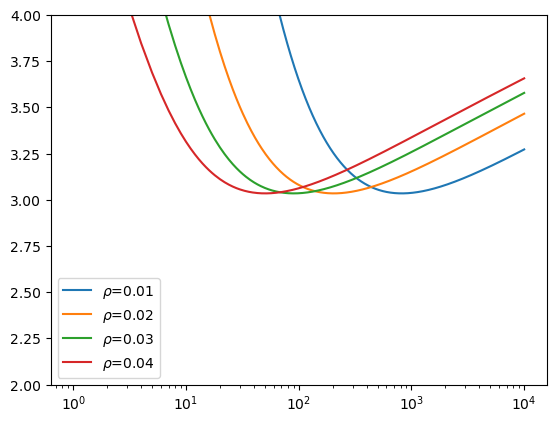
\includegraphics[width=.5\linewidth]{sprt.png}
    \caption{$u(t)/\sqrt{t}$ for various values of $\rho$}
    \label{fig:my_label}
\end{figure}

How do we choose $\rho$ ? Essentially the idea is given by Figure \ref{fig:}. Setting $u(t) = \sqrt{\frac{t + \rho^{-2}}{\rho^{-2}}\log\left(\frac{t+\rho^{-2}}{\rho^{-2} \delta^2}\right)}$, we have plotted $u(t)/\sqrt{t}$. Effectively, considering the normalized process $S_t/\sqrt{t}$, we want to choose $\rho$ so that the resulting boundary $u(t)/\sqrt{t}$ is minimized at an appropriate time $t_0$. In practice, this means that if you have the budget for a two week experiment, choose set $t_0$ appropriately and then solve for the value of $\rho$ which results in a curve pinching at $t_0$. See \cite{howard2021time} for more details. 


\noindent\textbf{Law of Iterated Logarithm.}

A natural question to ask is how to choose the tightest possible anytime confidence interval. As the discussion on the SPRT (and the MSPRT above) demonstrates, this question is not necessarily that meaningful - in practice we want to choose anytime intervals that are tight when we need them to be. A bound may be tight at a period of two weeks, but then be extremely loose after.  

Nevertheless, it's still reasonable to ask for the tightest possible anytime confidence interval \textit{asymptotically}. The answer to this is given by the law of the iterated logarithm.

\begin{theorem}
    Let $X_1, X_2, \cdots, $ be i.i.d. mean zero 1-subGaussian random variables. Then \[\lim\sup_{t\rightarrow \infty} \frac{S_t}{\sqrt{2t\log\log t}} = 1\] almost surely.
\end{theorem}

In general the LIL does not hold in finite time with a constant of 2. However, several works have provided finite time versions with slightly worse constants. The best one that I know of is from \cite{howard2021time} which shows,
\[\P(\exists t\leq 10^20: S_t\geq 1.7\sqrt{t(\log\log(e t) + 3.46)})\leq 0.025\]


\noindent \textbf{Anytime Inference in Linear Regression.} 

Imagine that we have collected a dataset $(x_1, y_1), \cdots, (x_n, y_n) \subset \mb{R}^d \times \mb{R}$ where $y_s = x_s^{\top}\theta + \epsilon_s$ where we assume $\epsilon_s$ is mean-zero $1$-sub-Gaussian noise. We also assume that $\{x_s\}_{s=1}^t$ form a \textit{fixed-design}, that is, we are assuming that the choice of $x_s$ is independent of the choice of $(x_1, y_1), \cdots, (x_{s-1}, y_s)$. 

For a minute we pretend that $\epsilon_s$ is exactly Gaussian noise with variance 1, and we assume that $V = \sum_{s=1}^t x_s x_s$ is invertible. Then recall the least-squares estimator,
\[\hat\theta_{\lambda} = \arg\min_{\theta' \in \mathbb{R}^d} \|Y - X\theta'\|^2_2, \hat{theta} = V^{-1} X^{\top} y\]
where $X = [x_1, \cdots, x_n]^{\top} \in \mathbb{R}^{n\times d}$ and $Y = [y_1, \cdots, y_n]\in\mathbb{R}^n$. 

We have that 
\begin{align*}
    \hat{\theta}
    &= V^{-1} X^{\top} y\\
    &= V^{-1} X^{\top} ( X\theta + \epsilon)\\
    &= \theta + V^{-1} X^{\top}\epsilon\\
    &= \theta + N(0, V^{-1})
\end{align*}

Thus $V^{1/2}(\hat{\theta} - \theta) \sim N(0, I)$ so that $\|\hat{\theta} - \theta\|_{V} \sim \chi^2_d$. We can now appeal to the Cramer-Chernoff method, note that for a $\chi^2_d$ random-variable, 
\begin{align*}
    
\end{align*}

We now relax the assumption that the sequence of observations is fixed in advance, and instead introduce the following assumptions
\begin{itemize}
    \item 
\end{itemize}

Now let's try this again. As above, let the least squares estimator by 
\begin{align*}
\hat{\theta} 
&= (V + \gamma I)^{-1} X^{\top}y  \\
&= (V + \lambd I)^{-1} V\theta +  (V + \lambda I)^{-1} \sum_{s=1}^t x_s\epsilon\\
&= (V + \lambda I)^{-1} V\theta +  (V + \lambda I)^{-1}M_t
\end{align*}

Now at the same time
\begin{align*}
\|\hat{\theta} - \theta\|_{V_t + \gamma I}
&= \|(V + \gamma I)^{-1} V\theta +  (V + \gamma I)^{-1}M_t - \theta\|_{V_t + \gamma I}\\
&= \|\gamma (V + \gamma I)^{-1} \theta +  (V + \gamma I)^{-1}S_t \|_{V_t + \gamma I}\\
&= \|\gamma \theta +  S_t \|_{(V_t + \gamma I)^{-1}}\\
&\leq \gamma\|\theta\|_{(V_t + \gamma I)^{-1}} + \|S_t\|_{(V_t + \gamma I)^{-1}}\\
&\leq \sqrt{\gamma}\|\theta\|_{2} + \|S_t\|_{(V_t + \gamma I)^{-1}}
\end{align*}

So the main game in town is $S_t$ - looking at it, if we could indeed conclude that the $x_s$'s were independent, standard concentration bounds would kick-in and we could easily bound it as above. However, we are allowing our sequences of $x_s$'s to be adaptive so we need a much more careful analysis. We will employ the ideas we used for the MSPRT.

To proceed, firstly note that for any $\psi\in \mathbb{R}^d$ that $M_t(\lambda) = \exp\left( \langle \lambda, S_t\rangle - \frac{\|\lambda\|_{V_t}^2}{2} \right)$ , 
where $V_t = \sum_{s=1}^t x_s x_s^{\top}$, is a super-Martingale. Then Ville's inequality automatically implies a linear boundary in this case, guaranteeing that $\P(\sup_{t\geq }\log(\bar{M}_t) \geq \log(1/\delta)) \leq \delta$

\exercise Check that $M_t$ forms a martingale sequence. 

Now, place a distribution $N(0, \gamma^{-1}I)$ over our choice of $\lambda$, and as we did with the MSPRT, we will now consider the Martingale $\bar{M}_t = \frac{1}{\sqrt{2\pi\gamma^{-d}}}\int M_t(\lambda) e^{-\frac{\|\lambda\|^2}{2\gamma^{-1}}} d\lambda$. We compute,
\begin{align*}
    \bar{M}_t 
    &= \frac{1}{\sqrt{2\pi\gamma^{-d}}}\int  e^{\langle\lambda, S_t\rangle -\frac{\|\lambda\|_{V + \gamma I}^2}{2}-\frac{\|\lambda\|^2\gamma}{2}} d\lambda\\
    &= \frac{1}{\sqrt{2\pi\gamma^{-d}}}\int e^{\frac{1}{2}\|S_t\|^2_(V_t + \gamma I)^{-1} - \frac{1}{2}\|(V_t + \gamma I)^{-1} S_t - \lambda\|^2_{V_t + \gamma I}} d\lambda\\
    &= \frac{|V_t + \gamma I|^{-1/2}}{\gamma^{-d/2}}\int e^{\frac{1}{2}\|S_t\|^2_(V_t +\gamma I )^{-1}} 
\end{align*}

Plugging this into our confidence inequality above, gives that with probability greater than $1-\delta$, for all $t\geq 0$
\[\|S_t\|_{V_t(\lambda)^{-1}} \leq \sqrt{2\log(1/\delta) + \log{\frac{|V_t + \gamma I|}{\gamma^d}}}\]

It remains to bound the second term under the square root. 



Firstly, we state the punch-line.




